\begin{frame}
    \frametitle{Difference between DHCP and static IP}
    \framesubtitle{In terms of energy consumption}

    \begin{columns}
        \begin{column}{0.5\textwidth}
            \begin{itemize}
                \item DHCP
                      \begin{itemize}
                          \item DHCP Server
                          \item IP addresses are allocated dynamically.
                          \item Lease-time
                      \end{itemize}
            \end{itemize}
        \end{column}
        \begin{column}{0.5\textwidth}
            \begin{itemize}
                \item Static IP address
                      \begin{itemize}
                          \item IP address stays static
                          \item DHCP server should know about this address
                          \item Be sure that the address is available
                      \end{itemize}
            \end{itemize}
        \end{column}
    \end{columns}
\end{frame}

\begin{frame}
    \frametitle{DHCP}
    \begin{columns}
        \begin{column}{0.5\textwidth}
            \begin{itemize}
                \item 4 steps required
                \item IP address is leased
                \item Renewal of the lease-time

            \end{itemize}
        \end{column}
        \begin{column}{0.5\textwidth}
            \begin{figure}
                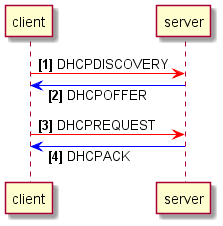
\includegraphics[scale=0.7]{../paper/fig/sequence_DHCP_connection.png}
            \end{figure}
        \end{column}
    \end{columns}
\end{frame}

\begin{frame}
    \frametitle{Experimental sequence: DHCP}
    \begin{figure}
        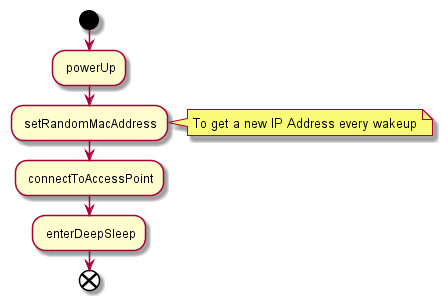
\includegraphics[scale=0.6]{../paper/fig/sequence_DHCP.png}
    \end{figure}
\end{frame}

\begin{frame}
    \frametitle{Experimental sequence: Statische IP}
    \begin{figure}
        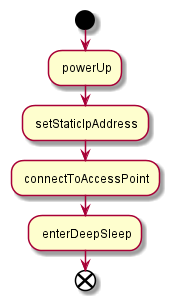
\includegraphics[scale=0.6]{../paper/fig/sequence_static_ip.png}
    \end{figure}
\end{frame}

\begin{frame}
    \frametitle{Results: DHCP}
    \begin{columns}
        \begin{column}{0.35\textwidth}
            \begin{itemize}
                \item $\overline{Duration}$: $\approx5.5s$
                \item $\overline{Consumption}$: $\approx0.35As$
                \item Only when the lease-time is expired
                \item Otherwise, roughly the same as using a static IP
            \end{itemize}
        \end{column}
        \begin{column}{0.65\textwidth}
            \begin{figure}
                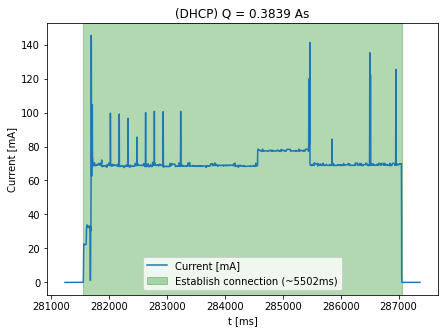
\includegraphics[scale=0.5]{../paper/fig/dhcp.png}
            \end{figure}
        \end{column}
    \end{columns}
\end{frame}

\begin{frame}
    \frametitle{Results: Static IP}
    \begin{columns}
        \begin{column}{0.35\textwidth}
            \begin{itemize}
                \item $\overline{Duration}$: $\approx4.0s$
                \item $\overline{Consumption}$: $\approx0.28As$
            \end{itemize}
        \end{column}
        \begin{column}{0.65\textwidth}
            \begin{figure}
                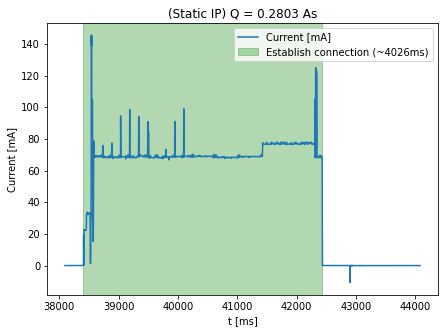
\includegraphics[scale=0.5]{../paper/fig/static_ip.png}
            \end{figure}
        \end{column}
    \end{columns}
\end{frame}

\begin{frame}
    \frametitle{Summary}

    \begin{itemize}

        \item The use of a static IP consumes $\approx 20.5\%$ less power
        \item Consumption when using DHCP depends on the lease-time
        \item Establishing the connection takes $\approx 1.5s$ longer when using DHCP and the lease-time is expired
        \item Example: \begin{itemize}
                  \item Lease-time = $50min$
                  \item Every $30min$ reconnect
                  \item Every second time, a new IP address is needed (Communication with DHCP server)
                  \item Leads to more power consumption
              \end{itemize}
    \end{itemize}


\end{frame}
